\documentclass{exam}
 
\usepackage{graphicx}
\usepackage{float}
\usepackage{amsmath}
\usepackage{subcaption}
\usepackage{algorithm2e}
 \usepackage{algpseudocode}
 
% First we setup the header and footer
\pagestyle{headandfoot}
\runningheadrule
\runningfootrule
\header{CSE101: Design and Analysis of Algorithms (CSE, UCSD, Summer-2020)}{}{Homework-02}
\footer{}{\thepage  \, of \numpages}{}
 
% We want the points for each question displayed on the left
%\pointname{points}
%\pointsinmargin
 
% Automatically total the points - make sure to compile TWICE
\addpoints
 
\begin{document}


\begin{center} 
\fbox{\parbox{5.5in}{
\vspace{-0.1in}
\begin{itemize}
\item \small{Unless otherwise mentioned, assume that graphs are given in adjacency list representation.}

\item \small{In the lectures, we have discussed an $O(V+E)$ algorithm for finding all the SCCs of a directed graph. We can extend this algorithm to design an algorithm {\tt CreateMetaGraph($G$)} that outputs the meta-graph of a given directed graph in $O(V+E)$ time. For this homework, you may use  {\tt CreateMetaGraph($G$)} as a sub-routine.}

\item \small{Other instructions are the same as in Homework-0 and Homework-1.}
\end{itemize}
\vspace{-0.1in}
}}
\end{center}

\vspace{0.1in}


\vspace{0.1in}
% Some general text together with number of questions and total points possible
There are \numquestions\, questions for a total of \numpoints\, points.
\vspace{0.1in}
\hrule
 \vspace{0.2in}
\begin{questions}
 
% First question, worth 3 points
\question  Consider the following directed graph and answer the questions that follow:

\begin{figure}[h]
\centering
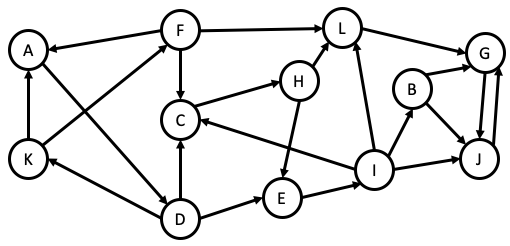
\includegraphics[scale=0.6]{scc}
\end{figure}

\begin{parts}
\part[1] Is the graph a DAG?\\ No

\part[2] How many SCCs does this graph have?\\ 5


\part[1] How many source SCCs does this graph have?\\ 1


\part[2] What is the distance of node $B$ from the $A$?\\ 4

\part[2] Suppose we run the DFS algorithm on the graph exploring nodes in alphabetical order. Given this, what is the pre-number of vertex $F$?\\ 20

\part[2] Suppose we run the DFS algorithm on the graph exploring nodes in alphabetical order. Given this, what is the post-number of vertex $G$?\\ 11
\end{parts}



\vspace{0.2in}



\question[20] Suppose a degree program consists of $n$ mandatory courses.
The {\em prerequisite graph} $G$ has a node for each course, and an edge from course $u$ to course $v$ if and only if $u$ is a prerequisite for $v$. Design an algorithm that takes as input the adjacency list of the prerequisite graph $G$ and outputs the minimum number of quarters necessary to complete the program. You may assume that there is no limit on the number of courses a student can take in one quarter. 
Analyse running time and give proof of correctness of your algorithm.\\

\begin{algorithm}
	\DontPrintSemicolon
	\SetKwFunction{FMain}{prereq}
	\SetKwProg{Fn}{procedure}{:}{}
	\Fn{\FMain{G}}{
		currPrereqs = getSources(G) \tcp*[f]{get source nodes, and indegree[] of all nodes}\\
		quarters = 0\\
		\While{currPrereqs is not empty}{
			quarters = quarters + 1\\
			nextPrereqs = empty list\\
			\ForAll{u in currPrereqs}{
				\ForAll{neighbors v of u}{
					indegree[v] = indegree[v] - 1\\
					\If{indegree[v] is 0}{
						add v to nextPrereqs\\
					}
				}
			}
			currPrereqs = nextPrereqs\\
		}
		\KwRet\ quarters\\
	}
\end{algorithm}

{\bf Correctness:}\\
The first courses we can take are the ones without any prerequisites. If these courses do not have any prerequisites, their indegrees must be 0, which means they are source nodes. We take all these source nodes for the first quarter, since we are trying to minimize graduation time. From here, we remove all the source nodes from the graph, and continue removing subsequent source nodes until every node has been traversed. The algorithm is correct because we do not traverse a node until ALL of its parents have been traversed. This ensures we are not accidentally skipping prerequisites when processing a node.\\


{\bf Running Time:}\\
The algorithm is essentially a modified BFS with constraints. A course is only added to the queue when it is a source node, meaning there is no other path to itself. Any graph-traversal algorithm at this point will never reach the node again, and will never process it again. This means that a course will never be added to the queue more than once. Given this property, we can guarantee that the runtime is not exponential, and is in fact the same as BFS, O(V + E).\\

The procedure getSources() was proven to have a runtime of O(V  + E) in HW1. Together, the entire algorithm has runtime O(V + E).\\

\vspace{0.2in}





\question[20] Given a strongly connected directed graph, $G = (V, E)$ with positive edge weights along with a particular node $v \in V$. 
You wish to pre-process the graph so that queries of the form ``what is the length of the shortest path from $s$ to $t$ that goes through $v$" can be answered in constant time for any pair of distinct vertices $s$ and $t$. The pre-processing should take the same asymptotic run-time as Dijkstra's algorithm. Analyse the runtime and provide a proof of correctness.\\

\leavevmode\newline
\leavevmode\newline
\leavevmode\newline
\leavevmode\newline
\leavevmode\newline
\begin{algorithm}
	\DontPrintSemicolon
	global distVtoT[] = empty array\\
	global distStoV[] = empty array\\
	\leavevmode\newline
	\SetKwFunction{FMain}{preprocess}
	\SetKwProg{Fn}{procedure}{:}{}
	\Fn{\FMain{G, $v_0$}}{
		setDist(G, $v_0$, distVtoT[])\\
		$G^\prime$ = reverseGraph(G)\\
		setDist($G^\prime$, $v_0$, distStoV[])\\
	}
	\leavevmode\newline
	\SetKwFunction{FMain}{setDist}
	\SetKwProg{Fn}{procedure}{:}{}
	\Fn{\FMain{G, $v_0$, dist[]}}{
		\ForAll{v in V}{
			dist[v] = $\infty$\\
		}
		dist[$v_0$] = 0\\
		Q = makeQueue(V)\\
		\While{Q is not empty}{
			u = deleteMin(Q)\\
			\ForAll{neighbors v of u}{
				\If{dist[u] + length(u,v) $<$ dist[v]}{
					dist[v] = dist[u] + length(u,v)\\
					decreaseKey(Q, v)\\
				}
			}
		}
	}
	\leavevmode\newline
	\SetKwFunction{FMain}{shortestPath}
	\SetKwProg{Fn}{procedure}{:}{}
	\Fn{\FMain{G, s, t}}{
		\KwRet\ distStoV[s] + distVtoT[t]\\
	}
\end{algorithm}

\leavevmode\newline
{\bf Correctness:}\\
Any shortest path from $s \rightarrow t$ must pass through $v$. Thus, this path must be of the form $s \rightarrow v \rightarrow t$. We can further break the problem down into 2 subproblems: finding the shortest path $s \rightarrow v$, and likewise for $v \rightarrow t$.\\

Finding the shortest paths from $v \rightarrow t$ is just a matter of running Dijkstra's algorithm on $v$. This computes the shortest distance from $v$ to any arbitrary $t$ in the graph.\\

Finding the shortest path from $s \rightarrow v$ is the same procedure, but we must first reverse the graph to get our path in the form $v \rightarrow s$. In this form, we only need to call our Dijkstra's algorithm once on $v$, and it will compute all shortest paths from $v \rightarrow s$, for any arbitrary $s$. Because the graph has been reversed, Dijkstra's algorithm is actually returning all the shortest paths from $s \rightarrow v$, which is what we are looking for.\\

The shortest path $s \rightarrow v \rightarrow t$ can now be computed by adding the shortest path $s \rightarrow v$ with the shortest path $v \rightarrow t$, for any arbitrary $s$ and $t$.\\

{\bf Running Time:}\\
The preprocess() procedure runs Dijkstra's algorithm twice, and also reverses the graph once. Dijkstra's algorithm has a runtime of O( (V + E) log V), and reversing a graph has a runtime of O(V + E), as shown in discussion. Together, preprocess() has worst-case runtime O( (V + E) log V).\\

The shortestPath() procedure is much simpler, and takes constant time O(1) to return the stored values of the shortest paths via array indexing.\\

\newpage



\question A particular  video game involves walking along some path in a map that can be represented as a directed graph $G = (V, E)$. 
At every node in the graph, there is a single bag of coins that can be collected on visiting that node for the first time. 
The amount of money in the bag at node $v$ is given by $c(v) > 0$.
The goal is to find what is the maximum amount of money that you can collect if you start walking from a given node $s \in V$.
The path along which you travel need not be a simple path. 

Design an algorithm for this problem. You are given a directed graph $G = (V, E)$ in adjacency list representation and a start node $s \in V$ as input. 
Also given as input is a matrix $C$, where $C[u] = c(u)$.
Your algorithm should return the maximum amount of money that is possible to collect when starting from $s$.
\begin{parts}
\part[15] Give a linear time algorithm that works for DAG's.\\

\part[10] Extend this to a linear time algorithm that works for any directed graph.
({\it \underline{Hint}: Consider making use of the meta-graph of the given graph.})
\end{parts}
Give running time analysis and proof of correctness for both parts.\\

\begin{parts}
\part
\begin{algorithm}
	\DontPrintSemicolon
	\SetKwFunction{FMain}{longestPathDAG}
	\SetKwProg{Fn}{procedure}{:}{}
	\Fn{\FMain{G, s, C[]}}{
		\ForAll{u in V}{
			dist[v] = $-\infty$\\
			prev[v] = nil\\
		}
		dist[s] = C[s]\\
		maxDist = C[s]\\
		Topologically sort G\\
		\For{node u = s to end of G, in linearized order}{
			\ForAll{neighbors v of u}{
				dist[v] = max(dist[v], dist[u] + C[v])\\
				distMax = max(distMax, dist[v])\\
			}
		}
		\KwRet\ distMax\\
	}
\end{algorithm}

{\bf Correctness:}\\
This problem is essentially asking us what is the length of the longest weighted path through a DAG. The weight of an edge $(u,v)$ is equivalent to the amount of money at node $v$, since this is the amount of money we collect immediately after traversing the edge.\\

The fact that $G$ is a DAG makes our life a lot less complicated. The constraint that our path need not be a simple path (meaning it can visit a node twice) immediately vanishes in a DAG. Every path in a DAG is a simple path, because it is {\em by definition} acyclic and cannot return to a visited node.\\

Once we have that contraint lifted, we now need to find the longest simple path in a DAG. We first topologically sort our DAG, such that the linear ordering of its nodes is preserved. Then, we consider how to find the longest path from $s$ to any other node . If there is path such that $s \rightarrow v \rightarrow t$, one must first compute the longest path from $s \rightarrow v$ before considering the longest edge to traverse from $v \rightarrow t$. Together, these will give us the longest path $s \rightarrow v \rightarrow t$.\\

Summarized, we need to find the longest paths from $s \rightarrow all\;of\;t's\;predecessors$ before we can find the longest path from $s \rightarrow t$. We can represent this in a recurrence relation as:\\

\begin{equation}
dist(v) = max\{dist(v), dist(u) + weight(v)\}\;for\;all\;edges\;(u,v)\;in\;E\\
\end{equation}

We can see how there are subproblems inside this equation, so we define our base case by setting the starting node $s$ to it's starting distance (money), $C[s]$. Now all we need to do is visit the nodes in linearized order, and update the edges out of each one, starting with $s$.\\

{\bf Running Time:}\\
The essence of the algorithm is running through all the nodes in linear order and updating every potential edge, which takes O(V + E) time.
Linearizing the graph itself takes O(V + E), and we run a loop through all nodes O(V) to initialize their distances. Therefore, the total runtime of this algorithm is linear. O(V + E)\\

\part
\begin{algorithm}
	\DontPrintSemicolon
	\SetKwFunction{FMain}{longestPathDirected}
	\SetKwProg{Fn}{procedure}{:}{}
	\Fn{\FMain{G, s, C[]}}{
		$G^\prime$ = CreateMetaGraph(G)\\
		\ForAll{SCC in $G^\prime$}{
			dist[SCC] = $-\infty$\\
			weight[SCC] = explore(SCC, a random node in SCC)
		}
		source = getSCC(s)\\
		dist[source] = weight[source]\\
		maxDist = weight[source]\\
		Topologically sort $G^\prime$\\
		\For{SCC curr =  source to end of $G^\prime$, in linearized order}{
			\ForAll{neighbors next of curr}{
				dist[next] = max(dist[next], dist[curr] + weight[next])\\
				distMax = max(distMax, dist[next])\\
			}
		}
		\KwRet\ distMax\\
	}
	\leavevmode\newline
	\SetKwFunction{FMain}{explore}
	\SetKwProg{Fn}{procedure}{:}{}
	\Fn{\FMain{SCC, u}}{
		visited[u] = true\\
		distNeighbors = 0\\
		\ForAll{neighbor v of u}{
			\If{not visited[v]}{
				distNeighbors += explore(SCC, v)\\
			}
		}
		\KwRet\ C[u] + distNeighbors\\
	}
\end{algorithm}

{\bf Correctness:}\\
The problem has changed, such that our input is no longer a DAG, which means it can have paths that contain cycles. However, we observe that we can obtain a DAG again by creating a {\em metagraph} of the given graph.\\

When we create a metagraph, we cluster the original graph into a collection of all its strongly connected components, or SCCs. These SCCs contain all the nodes which share a cycle with each other. Because these ``cyclic nodes'' are now clustered into their own SCCs, the resulting metagraph will essentially eliminate all cycles within the original graph. What we are left with is a DAG of SCCs.\\

Hopefully, it is already intuitive as to how we should operate on this metagraph. We can quite literally run $longestPathDAG()$ on this new DAG to achieve our solution. However, we must devise a way to calculate the weight of each SCC, since we are operating on SCCs now, not individual nodes.\\

The weight of an SCC is simply the sum of all nodes inside it, since there is guaranteed to be a path containing all nodes in an SCC, and we want to take the longest path. To account for this, we only need to run a modified DFS on an SCC. This DFS will keep a running count of the total weight of the SCC. It also fits the constraint that money will only be collected upon visiting a node for the first time, since DFS does not traverse already visited nodes.\\

Putting these together, we have effectively found a way to linearize any directed graph, and find the longest path from any arbitrary node $s$.\\

{\bf Running Time:}\\
The algorithm is the same as in $longestPathDirected()$, with the only exceptions being that we need to create our metagraph and get the weight of each SCC. Creating a metagraph takes O(V + E) time as stated in the homework. Getting the weight of each SCC is implemented through a modified DFS. A node cannot belong to multiple SCCs, so running DFS on all SCCs will only traverse each node once, O(V + E). Therefore, the entire algorithm is linear O(V + E).\\

\end{parts}

\vspace{0.3in}




\question Given a directed graph $G = (V, E)$ that is not a strongly connected graph, you have to determine if there exists a vertex that is reachable from every vertex in the graph. 
Design an algorithm for this problem. Your algorithm should output ``yes'' if such a vertex exists and ``no'' otherwise.
\begin{parts}
\part[15] Give a linear time algorithm that works for DAG's.

\part[10] Extend this to a linear time algorithm that works for any directed graph.
({\it \underline{Hint}: Consider making use of the meta-graph of the given graph.})
\end{parts}

Give running time analysis and proof of correctness for both parts.

\begin{parts}
\part
\begin{algorithm}
	\DontPrintSemicolon
	\SetKwFunction{FMain}{reachableDAG}
	\SetKwProg{Fn}{procedure}{:}{}
	\Fn{\FMain{G}}{
		$G^R$ = ReverseGraph(G)\\
		L = empty list\\
		L = getSources($G^R$)\\
		\If{size of L is 1}{
			\KwRet\ true\\
		}
		\Else{\KwRet\ false}
	}
\end{algorithm}

{\bf Correctness:}\\
We are trying to find out if there exists a node $u$ that is reachable by all other nodes in a DAG. First {\bf (Lemma 1)}, we will prove that if node $u$ does exist, it must be a sink node. We can do this through contradiction. Let's assume node $u$ exists, but is not a sink node. This means there is at least 1 outgoing edge from $u$, forming a path with any arbitrary node $v$. There is a path from $u \rightarrow v$. Node $u$ is reachable by every other node, so there must also be a path from $v \rightarrow u$. However, this breaks the property of a DAG, since there is now a cycle $u \leftrightarrow v$. Our assumption was false, and we can conclude that node $u$ must exist as a sink node.\\

Next {\bf (Lemma 2)}, we will prove that if a DAG contains precisely 1 sink node, that sink node has to be $u$. We will prove this through contradiction. Let's assume a DAG has 1 sink node $t$ without the special properties of $u$. This means it is not reachable from every node in the graph, or there are some nodes that do not have a path to $t$. If these nodes do not have a path to $t$, their paths must terminate in some other sink node. However, this breaks the assumption that our DAG only has 1 sink node. Thus we can conclude that if a DAG contains precisely 1 sink node, that sink node must $u$.\\

Lastly {\bf (Lemma 3)}, we will prove that a DAG containing $u$ cannot have any other sink nodes. We will prove this through contradiction. Let's assume a graph has 2 sink nodes, $u$ and $v$. Node $u$ has the special property, so there must be a path from $v \rightarrow u$. However, $v$ is also a sink node itself, and by definition cannot have any outgoing edges. Thus our assumption was false, and we can conclude that if $u$ exists, it must be the only sink node in the DAG.\\

From here, deriving an algorithm is simple. We only need to find the number of sink nodes in a DAG to conclude if $u$ exists or not. To do this, we simply reverse the graph, then find all its sources. Recall that sources and sinks switch characteristics when a graph is reversed, so we are actually finding the sink nodes in the original graph. Once we have found all the sink nodes, check if the number of sink nodes is 1. If it is, this sink node must be $u$. We have proven this in Lemma 2. Return true. Else, if the number of sink nodes is greater than 1, we know that neither of these sink nodes can be $u$. We have proven this in Lemma 3. Return false.\\

Note that the number of sink nodes cannot be less than 1, since by definition, every DAG has at least 1 sink node.\\

{\bf Running Time:}\\
The algorithm first reverses the DAG, which takes O(V + E) time. Then it gets all of it sources, which was proven to take O(V + E) time in HW1. Thus, our entire algorithm takes linear time O(V + E).\\

\part
\begin{algorithm}
	\DontPrintSemicolon
	\SetKwFunction{FMain}{reachableDirected}
	\SetKwProg{Fn}{procedure}{:}{}
	\Fn{\FMain{G}}{
		$G^R$ = ReverseGraph(G)\\
		$G^\prime$ = CreateMetaGraph($G^R$)\\
		L = empty list\\
		L = getSources($G^\prime$)\\
		\If{size of L is 1}{
			\KwRet\ true\\
		}
		\Else{\KwRet\ false}
	}
\end{algorithm}

{\bf Correctness:}\\
The issue of finding if $u$ exists in {\em any} directed graph is tougher, but can be remedied by reducing the directed graph to a DAG of SCCs. We find that Lemmas 1-3 apply to not only nodes, but also SCCs. Great! We can almost apply the previous algorithm to this metagraph. The only thing left to do is prove that if $u$ exists, it must be contained in the only sink SCC in the metagraph. This is trivial, because this sink SCC is the only SCC reachable by all SCCs in the metagraph. Since all nodes in an SCC are reachable to each other, it means that the nodes in this sink SCC are the only nodes reachable by all other nodes in the graph. Thus, $u$ must exist in this sink SCC.\\

{\bf Running Time:}\\
The algorithm is just the previous algorithm, but with the additional step of creating a metagraph. The runtime of creating a metagraph is given as O(V + E), so we conclude that the entire algorithm takes linear time O(V + E).\\

\end{parts}

\vspace{0.5in}











\end{questions}
\end{document}